% !TEX root = ../main.tex
\chapter{极限}

微积分之所以叫微积分，是因为它建立在两个核心概念之上：微分和积分。但是这两个概念都依赖于一个更根本的东西——\textbf{极限}。本章将正式引入极限的 $\epsilon-\delta$ 定义，这一章之后，希望你能用数学语言精确地描述“无限接近”这个概念。

\section{极限的 $\epsilon-\delta$ 定义}

极限的讨论对象是谁？是函数。所以我们必须先统一函数的概念。

\subsection{函数}

我们假定你在高中数学中学过函数。这里我们给出一个更精确的表述。

\begin{definition}{函数}{}
设有两个非空集合 $D$ 与 $Y$。若对于 $D$ 中的每一个元素 $x$，按照某种确定的对应法则 $f$，都有 $Y$ 中唯一确定的元素 $y$ 与之对应，则称 $f$ 是定义在 $D$ 上的一个\textbf{函数}，记作
\[
f: D \to Y, \quad y = f(x), \quad x \in D
\]
其中 $D$ 称为函数的\textbf{定义域}，全体函数值 $f(x)$ 构成的集合 $\{f(x) \mid x \in D\}$ 称为函数的\textbf{值域}。
\end{definition}

由此我们可以定义基本初等函数：
\begin{definition}{基本初等函数}{}
  以下六种函数统称为\textbf{基本初等函数}：

\textbf{常数函数}：\(f(x) = C\)（$C$为实常数）

\textbf{幂函数}：\(f(x) = x^{\mu} \quad (\mu \in \mathbb{R})\)

\textbf{指数函数}：\(f(x) = a^{x} \quad (a > 0,\ a \neq 1)\)

\textbf{对数函数}：\(f(x) = \log_{a} x \quad (a > 0,\ a \neq 1)\)

\textbf{三角函数}：\(\sin x,\ \cos x,\ \tan x,\ \cot x,\ \sec x,\ \csc x\)

\textbf{反三角函数}：\(\arcsin x,\ \arccos x,\ \arctan x,\ \operatorname{arccot} x,\ \operatorname{arcsec} x,\ \operatorname{arccsc} x\)

\end{definition}

更进一步，我们定义初等函数：

\begin{definition}{初等函数}{}
由基本初等函数经过有限次的四则运算和函数复合所构成的，并且可以用一个解析式表示的函数，称为\textbf{初等函数}。
\end{definition}

微积分讨论的都是初等函数，但实际上函数可以多种多样。例如著名的“狄利克雷函数”：有理数处取值为$1$，无理数处取值为$0$。

\[
D(x)=
\begin{cases}
  1,x\in \mathbb{Q} \\
  0,x\notin \mathbb{Q} 
\end{cases}
\]

它是一个极端的“病态”函数，处处不连续，处处不可导，处处不可积，甚至连图象都画不出来。但它确实是一个函数：$D=\mathbb{R} $，$Y=\{0,1\}$，对于 $D$ 中的每一个元素 $x$，都有 $Y$ 中唯一确定的元素 $y$ 与之对应。

1734 年，欧拉在著作中首次用 $f(x)$ 表示一个依赖于 $x$ 的量，这就是我们今天记号的来源。不过那时数学界理解的“函数”基本上就是“一条公式”，也就是必须有解析表达式才算函数。直到 1837 年，狄利克雷提出了现代函数的定义，也就是\textbf{只要每个 $x$ 对应唯一的 $y$，就是函数}。

接下来可以讨论极限了。在极限的讨论中，我们只关心 $x$ 无限接近某个 $x_0$ 时 $f(x)$ 的变化趋势。至于 $f(x_0)$ 本身是否存在、值是多少，我们并不在意。也就是说，极限只看重“趋近”的过程，不看“到达”的结果。

为了精确描述“接近某个点”这件事，我们需要先引入邻域的概念：

\begin{definition}{邻域}{}
设 $x_0$ 是数轴上的一个点，$\delta > 0$。则将集合
\[
U(x_0, \delta) = \{ x \mid |x - x_0| < \delta \} = (x_0 - \delta,\ x_0 + \delta)
\]
称为点 $x_0$ 的\textbf{$\delta$ 邻域}，其中$\delta$ 称为邻域的半径。
\end{definition}

简单来说，$x_0$ 的 $\delta$ 邻域就是以 $x_0$ 为中心、左右各延伸 $\delta$ 的一个开区间。

\begin{center}
  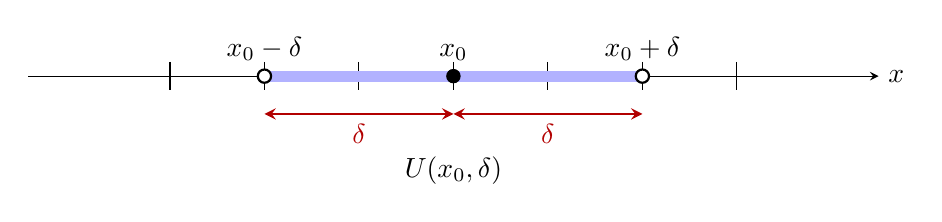
\begin{tikzpicture}[>=stealth, scale=1.2]

  % 数轴
  \draw[->] (-4.5,0) -- (4.5,0) node[right] {$x$};

  % 刻度线 (只画部分)
  \foreach \x in {-3,-2,-1,0,1,2,3}
    \draw (\x,0.15) -- (\x,-0.15);

  % 邻域区间的高亮 (可选)
  \draw[very thick, blue!30, line width=4pt, line cap=round] (-2,0) -- (2,0);

  % 中心点 x0 (实心)
  \filldraw (0,0) circle (2pt) node[above=2pt] {$x_0$};

  % 区间端点 (空心)
  \draw[fill=white, thick] (-2,0) circle (2pt) node[above=2pt] {$x_0-\delta$};
  \draw[fill=white, thick] (2,0) circle (2pt) node[above=2pt] {$x_0+\delta$};

  % 半径标注
  \draw[<->, red!70!black, thick] (0,-0.4) -- (2,-0.4) node[midway, below] {$\delta$};
  \draw[<->, red!70!black, thick] (-2,-0.4) -- (0,-0.4) node[midway, below] {$\delta$};

  % 邻域名称
  \node[below=0.9cm] at (0,0) {$U(x_0,\delta)$};

\end{tikzpicture}
\end{center}


邻域刻画的是“以 $x_0$ 为中心的一小段范围”。但在极限的讨论中，我们通常研究的是“趋近于 $x_0$ 时”会怎样，而不是“在 $x_0$ 处”怎样。所以我们反而并不关心 $x_0$ 这一点本身，于是我们去掉点 $x_0$，这就得到了去心邻域：

\begin{definition}{去心邻域}{}
设 $x_0$ 是数轴上的一个点，$\delta > 0$。则将集合
\[
\mathring{U}(x_0, \delta) = \{ x \mid 0 < |x - x_0| < \delta \} = (x_0 - \delta,\ x_0) \cup (x_0,\ x_0 + \delta)
\]
称为点 $x_0$ 的\textbf{$\delta$ 去心邻域}，其中$\delta$ 称为去心邻域的半径。

\end{definition}

去心邻域和邻域的唯一区别就是把 $x_0$ 本身挖掉了。

\begin{center}
  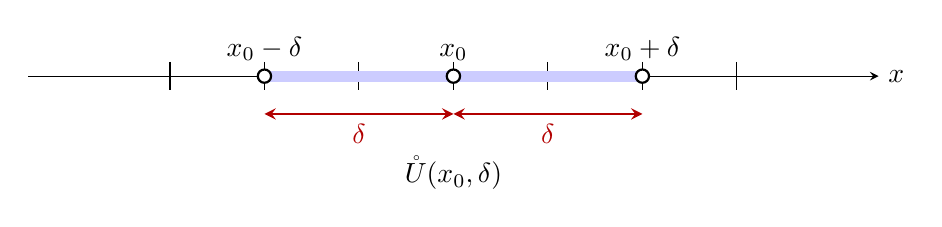
\begin{tikzpicture}[>=stealth, scale=1.2]
  
    % 数轴
    \draw[->] (-4.5,0) -- (4.5,0) node[right] {$x$};
  
    % 刻度线
    \foreach \x in {-3,-2,-1,0,1,2,3}
      \draw (\x,0.15) -- (\x,-0.15);
  
    % 邻域高亮（先画出整个区间，再通过覆盖实现挖空效果）
    \draw[very thick, blue!20, line width=4pt, line cap=round] (-2,0) -- (2,0);
  
    % 左端点 x0-δ（空心）
    \filldraw[fill=white, draw=black, thick] (-2,0) circle (2pt) node[above=2pt] {$x_0-\delta$};
    % 右端点 x0+δ（空心）
    \filldraw[fill=white, draw=black, thick] (2,0) circle (2pt) node[above=2pt] {$x_0+\delta$};
  
    % 中心点 x0（挖空，用稍大的空心圆表示）
    \filldraw[fill=white, draw=black, thick] (0,0) circle (2pt) node[above=2pt] {$x_0$};
  
    % 半径标注（左右两段长度均为 δ）
    \draw[<->, red!70!black, thick] (0,-0.4) -- (2,-0.4) node[midway, below] {$\delta$};
    \draw[<->, red!70!black, thick] (-2,-0.4) -- (0,-0.4) node[midway, below] {$\delta$};
  
    % 去心邻域符号
    \node[below=0.9cm] at (0,0) {$\mathring{U}(x_0,\delta)$};
  
  \end{tikzpicture}
\end{center}

有了邻域的语言，接下来我们可以用$\epsilon-\delta$语言来定义极限了。

\subsection{函数极限的 $\epsilon-\delta$ 定义}

先举一个简单的例子：设函数$f(x)=2x$，当 $x$ 越来越接近 $1$ 的时候，函数值越来越接近多少？显然是 $2$。也就是说，直觉上，当$x$ 无限接近 $1$ 时，$f(x)$ 无限接近 $2$。但问题来了，“无限接近”是个很模糊的词。到底是多近？用数学语言怎么描述？

我们先来玩一个游戏。假设你是一个水平极高的弓箭手，拥有一项技能，在相同位置射箭总能命中相同的位置，且已知$x_0$，在$x_0$射箭时总能精确地射中靶心 $y = L$，但在$x_0$附近射箭时会有偏差，不能精确射中靶心。然后我和你说，我指定一个$x_0$，你必须在距离$x_0$的$\delta$范围内射箭，而不是$x_0$，要求你射出的箭必须命中靶心区域，误差小于$\epsilon$，其中$\epsilon$是任意的，但是$x_0$不一定。我可以把$x_0$设在天上，地里，总之让你在$x_0$时无法射中靶心 $y = L$。虽然你水平很高，但是$x_0$的情况不清楚。这时你会怎么做？

让我们仔细想想。在距离$x_0$的$\delta$范围内，$\delta$是任意的。那么你可以说，没问题，但是我有个要求，$\delta$必须是我自己取的，而且$x_0$附近一定有我能射箭的地方。只要我找到一个$\delta$，能保证射出的箭就一定在$y = L$附近，且误差小于$\epsilon$，那么我就成功了。

按照这样的规定，游戏开始了。

我要求你在$x_0=1$处射箭，$\epsilon=1$。你说行，然后取了个$\delta=0.1$，射箭命中靶心附近，误差$0.99$，完美完成任务。我说不行，继续要求你在$x_0=999$处射箭，$\epsilon=0.0001$，你说没问题，然后取了个$\delta=0.00001$，射箭命中靶心附近，误差$0.00001$，完美完成任务。我说不行，我这次要求你在一万米高空中射箭，$\epsilon=0.001$，你说可以，然后找了一栋高楼，高度在$9999$米，接着你在天台射箭，命中靶心附近，误差$0.0009$，完美完成任务。

也就是说，无论我给什么$x_0$和$\epsilon $，只要能找到一个$\delta$，使得射出的箭距离靶心永远在$\epsilon$误差范围内，那么你就赢了。

我们把概念抽象一下。我们把“必须在距离$x_0$的$\delta$范围内射箭，而不是$x_0$”叫做“点 $x_0$ 的某个去心邻域内”，把“$x_0$附近一定有我能射箭的地方”叫做“函数 $f(x)$ 在点 $x_0$ 的某个去心邻域内有定义”，那么我们就可以给出极限的定义：

\begin{definition}{函数极限的 $\epsilon-\delta$ 定义}{}
设函数 $f(x)$ 在点 $x_0$ 的某个去心邻域内有定义，$L$ 是一个实数。若对于任意给定的 $\epsilon > 0$，总存在 $\delta > 0$，使得当
\[
0 < |x - x_0| < \delta
\]
时，一定有
\[
|f(x) - L| < \epsilon
\]
则称当 $x$ 趋近于 $x_0$ 时，$f(x)$ 的\textbf{极限}为 $L$ ，记作
\[
\lim_{x \to x_0} f(x) = L
\]
\end{definition}

也就是说，无论$x_0$取什么值，只要$x_0$ 的某个去心邻域内有定义，即使函数在$x_0$ 处无定义，只要满足上面的条件，那么我们也能求出函数的极限。

从图中可以看出，$f(x)$ 在 $\mathring{U}(x_0, \delta)$ 内的所有函数值都落在 $U(L, \epsilon)$ 内。这就是极限的几何表示。


\begin{center}
  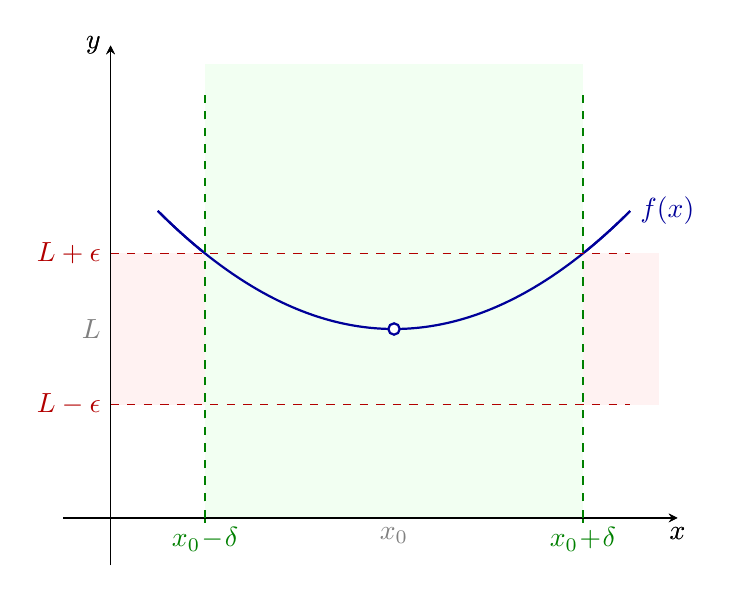
\begin{tikzpicture}[>=stealth, scale=1.2]
  
  % --- 坐标轴 ---
  \draw[->] (-0.5,0) -- (6,0) node[below] {$x$};
  \draw[->] (0,-0.5) -- (0,5) node[left] {$y$};
  
  % --- 函数曲线 (例如 f(x)=0.2*(x-3)^2+2) ---
  \draw[domain=0.5:5.5, samples=100, thick, blue!60!black]
      plot (\x, {0.2*(\x-3)^2 + 2}) node[right] {$f(x)$};
  
  % --- 极限点 x0, L ---
  \def\xo{3}
  \def\L{2}
  
  % x0 处画虚线确定 L
  \draw[dashed, gray] (\xo, 0) node[below] {$x_0$} -- (\xo, \L);
  
  % 在 x0 处画空心圆 (去心邻域)
  \filldraw[fill=white, draw=blue!60!black, thick] (\xo, \L) circle (0.06);
  
  % y=L 的标记
  \draw[dashed, gray] (0, \L) node[left] {$L$} -- (\xo, \L);
  
  % --- 定义 epsilon = 0.8, 则 L ± epsilon ---
  \def\eps{0.8}
  \draw[dashed, red!70!black] (0, \L+\eps) node[left] {$L+\epsilon$} -- (5.5, \L+\eps);
  \draw[dashed, red!70!black] (0, \L-\eps) node[left] {$L-\epsilon$} -- (5.5, \L-\eps);
  
  % 标注 epsilon 的双向箭头
  \draw[<->, red!70!black] (5.3, \L) -- (5.3, \L+\eps) node[midway, right] {$\epsilon$};
  \draw[<->, red!70!black] (5.3, \L) -- (5.3, \L-\eps) node[midway, right] {$\epsilon$};
  
  \def\del{2} % delta=2
  % 竖直线 x0±delta
  \draw[dashed, green!50!black] (\xo-\del, 0) -- (\xo-\del, 4.5);
  \draw[dashed, green!50!black] (\xo+\del, 0) -- (\xo+\del, 4.5);
  
  % 标注 delta 的双向箭头
  \draw[<->, green!50!black] (\xo-\del, 1.2) -- (\xo, 1.2) node[midway, above] {$\delta$};
  \draw[<->, green!50!black] (\xo, 1.2) -- (\xo+\del, 1.2) node[midway, above] {$\delta$};
  
  % 在 x 轴上标出区间
  \draw[green!50!black, thick] (\xo-\del, 0.05) -- (\xo-\del, -0.05);
  \draw[green!50!black, thick] (\xo+\del, 0.05) -- (\xo+\del, -0.05);
  \node[below, green!50!black] at (\xo-\del, 0) {$x_0\!-\!\delta$};
  \node[below, green!50!black] at (\xo+\del, 0) {$x_0\!+\!\delta$};
  
  % --- 填充区间背景，强调带子 ---
  % 水平 epsilon 带
  \fill[red!5] (0, \L-\eps) rectangle (5.8, \L+\eps);
  % 竖直 delta 带（去心，但这里无法方便地打洞，我们覆盖上去）
  \fill[green!5] (\xo-\del, 0) rectangle (\xo+\del, 4.8);
  
  % 重新绘制轴和曲线，以确保它们在最上层
  \draw[->] (-0.5,0) -- (6,0) node[below] {$x$};
  \draw[->] (0,-0.5) -- (0,5) node[left] {$y$};
  \draw[domain=0.5:5.5, samples=100, thick, blue!60!black]
      plot (\x, {0.2*(\x-3)^2 + 2});
  
  % 再次画出 L±eps 的虚线, x0±delta 虚线等，以免被填充覆盖
  \draw[dashed, red!70!black] (0, \L+\eps) -- (5.5, \L+\eps);
  \draw[dashed, red!70!black] (0, \L-\eps) -- (5.5, \L-\eps);
  \draw[dashed, green!50!black] (\xo-\del, 0) -- (\xo-\del, 4.5);
  \draw[dashed, green!50!black] (\xo+\del, 0) -- (\xo+\del, 4.5);
  
  % 重描空心点
  \filldraw[fill=white, draw=blue!60!black, thick] (\xo, \L) circle (0.06);
  
  \end{tikzpicture}
\end{center}

我们理解一下这个定义：

$\epsilon$是我指定的误差范围，也就是我要求你的箭必须落在离靶心 $L$ 小于 $\epsilon$ 的范围内。$\epsilon$ 越小，我对你精度的要求就越苛刻。

$\delta$是你找的射箭范围，只要你在离 $x_0$ 小于 $\delta$ 的范围内选一个位置射箭，你就保证命中。$\epsilon$ 越小，你选的 $\delta$ 通常也得越小。

$0 < |x - x_0|$意味着不能在 $x_0$ 本身射箭，$x_0$ 可能在天上、在地里、在墙里面，总之你没法站在 $x_0$ 那个点上射箭。你只能在 $x_0$ 附近选位置。翻译成数学语言就是 $x \neq x_0$，极限只看附近的表现，不管 $x_0$ 本身什么情况，即使函数在$x_0$处无定义。

$|x - x_0| < \delta$就是说你的射箭位置必须在 $\delta$ 范围内。

$|f(x) - L| < \epsilon$是射出去的箭必须命中的靶心范围，$f(x)$ 是落点的坐标。这个落点必须距离 $L$ 小于 $\epsilon$。


这个游戏的胜负标准就是：\textbf{无论我给出多小的 $\epsilon$，你都能找到一个 $\delta$，保证在距离$x_0$的$\delta$ 范围内的每一次射箭，最终都落在距离靶心$L$的$\epsilon$ 范围内。}一旦你找到了这样的 $\delta$，我就承认 $\lim_{x \to x_0} f(x) = L$。

用数学符号，极限的定义可以写成：

\begin{center}
  \(\forall \epsilon > 0\)，
  \(\exists \delta > 0\)，使得\(0 < |x - x_0| < \delta \)，\(|f(x) - L| < \epsilon\)恒成立，则有\(\lim_{x \to x_0} f(x) = L\)
\end{center}

只需要对每个 $\epsilon$ 分别找到一个 $\delta$即可，$\delta$ 可以随着 $\epsilon$ 的改变而改变。

接下来我们再看看我们最开始举的例子：

\begin{myexample}
  举例说明：用 $\epsilon-\delta$ 定义证明 $\lim\limits_{x \to 1}2x = 2$。

  我们先回忆一下定义：对任意给定的 $\epsilon > 0$，都存在 $\delta > 0$，使得当 $0 < |x - x_0| < \delta$ 时，$|f(x) - L| < \epsilon$。

  也就是说，我们要证明的是，对任意给定的 $\epsilon > 0$，都存在 $\delta > 0$，使得当 $0 < |x - 1| < \delta$ 时，$|2x - 2| < \epsilon$。

  那么假设我们现在就是弓箭手，现在我们的目标就是找到一个$\delta > 0$，使得当 $0 < |x - 1| < \delta$ 时，$|2x - 2| < \epsilon$。

  要让 $|2x - 2| < \epsilon$，也就是$2|x - 1| < \epsilon$，只需 $|x - 1| < \frac{\epsilon}{2}$。因此取 $\delta < \frac{\epsilon}{2}$ 即可。

  那么我们不妨取$\delta = \frac{\epsilon}{3}$，那么我们可以得到这样的证明：

对任意的 $\epsilon > 0$，取 $\delta = \frac{\epsilon}{3}$。则当 $0 < |x - 1| < \delta$ 时，有：
\[
|2x - 2| = 2|x - 1| < 2\delta = \frac{2\epsilon}{3} < \epsilon
\]

由 $\epsilon-\delta$ 定义，$\lim\limits_{x \to 1} 2x = 2$。

\end{myexample}

我们用射箭游戏说明，就是我给出了任意的 $\epsilon$，你算出了 $\delta < \frac{\epsilon}{2}$，并取了$\delta = \frac{\epsilon}{3}$，然后在 $x_0=1$ 的 $\delta$ 去心邻域内任意位置射箭，每一箭的落点 $f(x)$ 都落在距离 $L=2$ 小于 $\epsilon$ 的范围内。游戏获胜。

总结一下：

先根据$|f(x) - L| < \epsilon$求出$\delta$的范围。

然后在$\delta$的范围内取一个合适的$\delta$。

代入定义，得到证明。

当然这只是简单的极限证明。我们了解即可，具体的使用那是数学分析才做的事情，更深入的我们这里不作讨论。

\section{极限的性质}

有了 $\epsilon-\delta$ 定义这个工具，我们可以严格地讨论极限的各种性质了。这些性质会在后续计算极限时用到，但是计算极限本身不是我们的重点，因此这里简单带过。

\subsection{单侧极限}

有时，函数在 $x_0$ 的两侧表现不同，比如分段函数在分段点处，如果还用$x_0$的$\delta $邻域定义极限，会发现两边的定义完全不同。这时我们就要区分“从左边趋近”和“从右边趋近”。

因此，我们就引出了左极限与右极限：

\begin{definition}{左极限与右极限}{}
设函数 $f(x)$ 在 $x_0$ 的左侧某个区间 $(x_0 - \delta_0,\ x_0)$ 内有定义，$L$ 为实数。

\textbf{左极限}：若对任意 $\epsilon > 0$，存在 $\delta > 0$，使得当 $x_0 - \delta < x < x_0$ 时，$|f(x) - L| < \epsilon$，则称 $L$ 为 $f(x)$ 在 $x_0$ 处的\textbf{左极限}，记作
\[
\lim_{x \to x_0^-} f(x) = L \quad \text{或} \quad f(x_0^-) = L
\]

设函数 $f(x)$ 在 $x_0$ 的右侧某个区间 $(x_0,\ x_0 + \delta_0)$ 内有定义，$L$ 为实数。

\textbf{右极限}：若对任意 $\epsilon > 0$，存在 $\delta > 0$，使得当 $x_0 < x < x_0 + \delta$ 时，$|f(x) - L| < \epsilon$，则称 $L$ 为 $f(x)$ 在 $x_0$ 处的\textbf{右极限}，记作
\[
\lim_{x \to x_0^+} f(x) = L \quad \text{或} \quad f(x_0^+) = L
\]
\end{definition}

左极限就是只看 $x_0$ 左边的点，右极限就是只看 $x_0$ 右边的点。用射箭游戏的比喻就是，左极限是只允许你在 $x_0$ 的左侧射箭，右极限是只允许你在 $x_0$ 的右侧射箭。

单侧极限最常见的应用场景就是分段函数在分段点处的极限问题。先分别求左右极限，再看它们是否相等，判断函数是否在该点处有极限。

\begin{myexample}
  设 $f(x) = |x|$，求 $\lim\limits_{x \to 0} f(x)$。

  当 $x < 0$ 时， $f(x) = -x$，因此 $\lim\limits_{x \to 0^-} |x| = \lim\limits_{x \to 0^-} -x = 0$。

  当 $x > 0$ 时， $f(x) = x$，因此 $\lim\limits_{x \to 0^+} |x| = \lim\limits_{x \to 0^+} x = 0$。

  左右极限都等于 $0$，故 $\lim\limits_{x \to 0} |x| = 0$。
\end{myexample}

\begin{myexample}
  设 $f(x) = \begin{cases} x+1, & x \geq 0 \\ x-1, & x < 0 \end{cases}$，讨论 $\lim\limits_{x \to 0} f(x)$。

  左极限：$\lim\limits_{x \to 0^-} f(x) = \lim\limits_{x \to 0^-} x-1 = -1$。

  右极限：$\lim\limits_{x \to 0^+} f(x) = \lim\limits_{x \to 0^+} x+1 = 1$。

  然而$-1 \neq 1$，即左右极限不相等，故 $\lim\limits_{x \to 0} f(x)$ 不存在。
\end{myexample}

也就是说，函数在一点有极限，就是在该点的左右极限都存在且相等，否则就说函数在这一点极限不存在。

\begin{theorem}{极限与单侧极限的关系}{}
函数在一点处极限存在的充要条件是该点左右极限都存在且相等。即：

  \begin{center}
    若\(\lim_{x \to x_0^-} f(x) = \lim_{x \to x_0^+} f(x) = L\)，则\(\lim_{x \to x_0} f(x) = L\)
  \end{center}

  反之亦成立。

\end{theorem}

\subsection{无穷远处的极限}

极限不仅关心 $x$ 趋近于某个有限点 $x_0$，也关心 $x$ 无限增大或无限减小时 $f(x)$ 的趋势。例如 $\lim\limits_{x \to \infty} \frac{1}{x} = 0$，当 $x$ 越来越大时，$\frac{1}{x}$ 越来越接近 $0$。那么我们就可以引出无穷远处的极限：

\begin{definition}{自变量趋于无穷时的极限}{}
设函数 $f(x)$ 当 $|x|$ 大于某个正数时有定义，$L$ 为实数。若对任意 $\epsilon > 0$，存在 $X > 0$，使得当 $|x| > X$ 时，$|f(x) - L| < \epsilon$，则称当 $x$ 趋于无穷大时，$f(x)$ 的极限为 $L$，记作
\[
\lim_{x \to \infty} f(x) = L
\]

其中，把 $|x| > X$ 换成 $x > X$，则得到 $x \to +\infty$ 时的极限；换成 $x < -X$，则得到 $x \to -\infty$ 时的极限。
\end{definition}

这里的结构和 $\epsilon-\delta$ 定义完全平行：$\epsilon$ 仍然控制函数值的精度，而 $\delta$ 的角色被 $X$ 取代。$X$ 控制的是自变量“离开原点”的距离。$\epsilon$ 越小，$X$ 通常需要越大。

在符号表示上，用箭头方向加以区分：
\[
\lim_{x \to +\infty} f(x) = L, \qquad \lim_{x \to -\infty} f(x) = L, \qquad \lim_{x \to \infty} f(x) = L
\]

和单侧极限一样，只有当\(\lim_{x \to +\infty} f(x) = \lim_{x \to -\infty} f(x) = L\)时，才能说\(\lim_{x \to \infty} f(x) = L\)。

让我们回到一开始的那个$\lim\limits_{x \to \infty} \frac{1}{x} = 0$的例子：

\begin{myexample}
  证明$\lim\limits_{x \to \infty} \frac{1}{x} = 0$。

  对任意 $ \epsilon>0$，要使 $| \frac {1}{x} -0|< \epsilon $ ，只需$|x|> \frac {1}{\epsilon } $ ，因为$|x| > X$，取$X= \frac {2}{\epsilon } $ 即可。

  所以对任意的$\epsilon >0$，取$ X= \frac {2}{\epsilon }$。则当$|x|>X$时，有：
  \[|\frac{1}{x}-0|=\frac{1}{|x|}<\frac{1}{X}=\frac {\epsilon }{2}<\epsilon \]

  由$\epsilon-X$ 定义，$\lim\limits_{x \to \infty} \frac{1}{x} = 0$。
\end{myexample}

\subsection{运算律}

如果每次求极限都要从 $\epsilon-\delta$ 定义出发，那就太麻烦了。幸好，极限满足一系列运算律，使得我们可以像做加减乘除一样计算极限。

\begin{theorem}{极限的四则运算法则}{}
若 $\lim\limits_{x \to x_0} f(x) = A$，$\lim\limits_{x \to x_0} g(x) = B$，其中$A$，$B$ 均为有限实数，则
\[
\begin{aligned}
&\text{(1)}\ \lim_{x \to x_0} [f(x) \pm g(x)] = A \pm B
&&\text{(2)}\ \lim_{x \to x_0} [f(x) \cdot g(x)] = A \cdot B \\[4pt]
&\text{(3)}\ \lim_{x \to x_0} [c\,f(x)] = c\,A \quad (c\text{ 为常数})
&&\text{(4)}\ \lim_{x \to x_0} \frac{f(x)}{g(x)} = \frac{A}{B} \quad (B \neq 0)
\end{aligned}
\]
\end{theorem}

简单来说就是：\textbf{极限可以加减乘除}，和的极限等于极限的和，积的极限等于极限的积，商的极限等于极限的商（分母极限不为零）。这些法则对 $x \to \infty$ 以及单侧极限也同样成立。

还有一个非常实用的工具叫夹逼定理：

\begin{theorem}{夹逼定理}{}
若在 $x_0$ 的某个去心邻域内，$g(x) \leq f(x) \leq h(x)$，且
\(\lim_{x \to x_0} g(x) = \lim_{x \to x_0} h(x) = L\)，
则\(\lim_{x \to x_0} f(x) = L\)。
\end{theorem}

夹逼定理的思想很简单：$f(x)$ 被 $g(x)$ 和 $h(x)$ 两个函数“夹”在中间，而这两个极限都趋向同一个值 $L$，那么中间的 $f(x)$ 别无选择，也只能趋向 $L$。不过本章中，我们不会对如何求极限作详细说明，因为我们的重点是微积分。

\subsection{无穷小量与无穷大量}

有了极限的定义，我们可以严格地讨论“小到几乎为零的量”和“大到没有上界的量”。

\begin{definition}{无穷小量}{}
若 $\lim\limits_{x \to x_0} f(x) = 0$（或 $x \to \infty$ 时），则称 $f(x)$ 为该极限过程中的一个\textbf{无穷小量}。
\end{definition}

类似地，我们有：

\begin{definition}{无穷大量}{}
若对任意 $M > 0$，存在 $\delta > 0$（或 $X > 0$），使得当 $0 < |x - x_0| < \delta$（或 $|x| > X$）时，$|f(x)| > M$，则称 $f(x)$ 为该极限过程中的一个\textbf{无穷大量}，记作
\[
\lim_{x \to x_0} f(x) = \infty
\]
\end{definition}

需要注意的是，无穷小量不是“一个很小的数”，而是在极限过程中，绝对值可以小于任何预先给定的正数 $\epsilon$ 的量。$0 $是唯一可以称为无穷小量的常数。因此，趋于无穷小也说成趋于零。同理，无穷大量不是“一个很大的数”，也不是一个确定的数，所以当我们说极限趋于无穷大时，这个极限其实是不存在的。

我们举个例子：

\begin{myexample}
  验证 $\lim\limits_{x \to +\infty} x^2 = +\infty$。

  对任意 $M > 0$，取 $X = \sqrt{M}$。当 $x > X$ 时，$x^2 > X^2 = M$。所以 $\lim_{x \to +\infty} x^2 = +\infty$。
\end{myexample}

也就是说，当$x \to +\infty$时，$x^2 \to +\infty$，极限不存在。

无穷大量和无穷小量之间有一个简洁的倒数关系：

\begin{theorem}{无穷大与无穷小的关系}{}
在同一极限过程中：

1.若 $f(x)$ 是无穷小量且 $f(x) \neq 0$，则 $\frac{1}{f(x)}$ 是无穷大量。

2.若 $f(x)$ 是无穷大量，则 $\frac{1}{f(x)}$ 是无穷小量。

\end{theorem}

这个关系非常直观，把几乎为零的数倒过来，就变成大到没边的数，反之亦然。

有时我们需要比较两个无穷小量“谁小得更快”，这就引出了无穷小量的阶的概念：

\begin{definition}{无穷小量的阶}{}
设 $\alpha(x)$ 和 $\beta(x)$ 都是 $x \to x_0$ 时的无穷小量，且当 $x \neq x_0$ 时， $\beta(x) \neq 0$。定义极限
\(
\lim_{x \to x_0} \frac{\alpha(x)}{\beta(x)}
\)：

1.若$\lim_{x \to x_0} \frac{\alpha(x)}{\beta(x)}
=0$，则称 $\alpha$ 是比 $\beta$ \textbf{高阶}的无穷小，记作 $\alpha = o(\beta)$。

2.若$\lim_{x \to x_0} \frac{\alpha(x)}{\beta(x)}
=c$，其中$c \neq 0$且为常数，则称 $\alpha$ 与 $\beta$ 是\textbf{同阶}无穷小。

3.若$\lim_{x \to x_0} \frac{\alpha(x)}{\beta(x)}
=1$，则称 $\alpha$ 与 $\beta$ 是\textbf{等价}无穷小，记作 $\alpha \sim \beta$。

4.若$\lim_{x \to x_0} \frac{\alpha(x)}{\beta(x)}
=\infty$，则称 $\alpha$ 是比 $\beta$ \textbf{低阶}的无穷小。此时 $\beta$ 就是比 $\alpha$ 高阶的无穷小，即 $\beta = o(\alpha)$。

5.若$\lim_{x \to x_0} \frac{\alpha(x)}{[\beta(x)]^k}=c$，其中$c \neq 0$且为常数，则称 $\alpha$ 是关于$\beta$的 \textbf{$k$ 阶}无穷小。通常以$\beta (x) = x-x_0$为基准，称 $\alpha$ 是$x$的\textbf{$k$ 阶}无穷小。

\end{definition}

越高阶的无穷小，趋向于$0 $的速度就越快。$0 $通常被视为“最高阶”的无穷小，没有比$ 0 $更高阶的无穷小了。

其中，最常用的是等价无穷小。等价无穷小在求极限时非常有用，只要是乘除运算，就可以把一个等价无穷小替换成另一个，大大简化计算。

\section{函数的连续性}

极限只关心 $x$ 趋近于 $x_0$ 时 $f(x)$ 的趋势，不关心 $f(x_0)$ 本身。现在我们把视线拉回来，同时看“趋近”和“在点处”，如果这两者能对上，我们就说函数在这一点是连续的。连续性是比极限存在更“强”的性质。

\subsection{连续的不同定义}

历史上数学家从多个角度描述“连续”，最终它们被证明是等价的。我们先给出最标准的 $\epsilon-\delta$ 定义。

\begin{definition}{函数在一点处的连续性}{}
设函数 $f(x)$ 在 $x_0$ 的某个邻域内有定义。若对任意 $\epsilon > 0$，存在 $\delta > 0$，使得当 $|x - x_0| < \delta$ 时，有
\[
|f(x) - f(x_0)| < \epsilon
\]
则称 $f(x)$ 在点 $x_0$ 处\textbf{连续}。
\end{definition}

对比极限的定义，连续性只改了两处：不再挖掉 $x_0$，把极限值 $L$ 换成了函数值 $f(x_0)$。换句话说：

\begin{theorem}{连续与极限的关系}{}
$f(x)$ 在 $x_0$ 处连续是$\lim\limits_{x \to x_0} f(x) = f(x_0)$的充要条件。

\end{theorem}

这个关系暗含了函数在某一点连续的三个条件：极限存在、函数值存在、两者相等。这三者缺一不可。任何一条不满足，我们就说函数在 $x_0$ 处间断。由此引出间断点的定义：

\begin{definition}{间断点}{}
  若函数$f(x)$在点$x_0$不连续，则称$x_0$为该函数的间断点。
\end{definition}

用$\epsilon-\delta$ 定义函数的连续是现代数学分析的基石。如果我们在直观上理解，还可以用“增量”定义连续：令 $\Delta x = x - x_0$（自变量的微小变化），$\Delta y = f(x_0 + \Delta x) - f(x_0)$（函数值的相应变化），则函数的连续性等价于：
\[
\lim_{\Delta x \to 0} \Delta y = 0
\]

也就是说，如果自变量的微小变化只引起函数值的微小变化，我们就说这个函数连续。这个定义实际上与$\epsilon-\delta$ 定义是等价的。

和单侧极限类似，我们有单侧连续：

\begin{definition}{左连续与右连续}{}
若 $\lim\limits_{x \to x_0^-} f(x) = f(x_0)$，则称 $f(x)$ 在 $x_0$ 处\textbf{左连续}。

若 $\lim\limits_{x \to x_0^+} f(x) = f(x_0)$，则称 $f(x)$ 在 $x_0$ 处\textbf{右连续}。

\end{definition}

同理可得，$f(x)$ 在 $x_0$ 处连续的充要条件是$f(x)$在 $x_0$ 处既左连续又右连续。

\begin{theorem}{连续与单侧连续的关系}{}
  函数在一点处连续的充要条件是函数在该点左右都连续。即：

  \begin{center}
    若\(\lim_{x \to x_0^-} f(x) = \lim_{x \to x_0^+} f(x) = f(x_0)\)，则\(f(x)\)在\(x_0\)处连续。
  \end{center}

  反之亦成立。

\end{theorem}

根据“哪里不连续”，我们可以对间断点进行分类：

\begin{definition}{间断点的分类}{}
设 $x_0$ 是 $f(x)$ 的间断点。

\textbf{第一类间断点}：左右极限都存在。其中：

若左右极限相等，则称 $x_0$ 为\textbf{可去间断点}。

若左右极限不相等，则称 $x_0$ 为\textbf{跳跃间断点}，差值 $|f(x_0^+) - f(x_0^-)|$ 称为\textbf{跃度}。

\textbf{第二类间断点}：左右极限中至少有一个不存在。
\end{definition}

\begin{myexample}
  判断$f(x) = |x|$ 在 $x=0$ 处的连续性。

  我们先回忆一下连续的三个条件：极限存在、函数值存在、两者相等。

  先看极限存不存在。计算左右极限：

  左极限：
\[
\lim_{x \to 0^-} |x| = \lim_{x \to 0^-}-x= 0
\]

右极限：
\[
\lim_{x \to 0^+} |x| = \lim_{x \to 0^+}x= 0
\]

左极限等于右极限，因此函数在$x=0$ 处极限存在，也就是：
\[
\lim_{x \to 0} |x| =0
\]

再看函数值：
\[
f(0) = 0
\]

极限和函数值相等。三个条件都满足，因此$f(x) = |x|$ 在 $x=0$ 处连续。

\end{myexample}

\begin{myexample}
    判断分段函数 $f(x) = \begin{cases} x+1, & x \geq 0 \\ x-1, & x < 0 \end{cases}$ 在 $x=0$ 处的连续性。

    我们同样先计算极限：

    左极限：
\[
\lim_{x \to 0^-} f(x) = \lim_{x \to 0^-} (x-1) = -1
\]

右极限：
\[
\lim_{x \to 0^+} f(x) = \lim_{x \to 0^+} (x+1) = 1
\]

左右极限不相等，因此$f(x)$ 在 $x=0$ 处不连续。

更进一步的，$x=0$是函数 $f(x)$ 的跳跃间断点，跃度为$2$。
\end{myexample}

在这一章最开始，我们提到了狄利克雷函数 $D(x)$ ，它就是一个处处不连续的函数，在任何点的任何邻域内，函数值在 $0$ 和 $1$ 之间不断跳变，极限根本不存在。这是第二类间断点的极端例子。

\subsection{闭区间上连续函数的性质}

闭区间上的连续函数具有几条非常“舒服”的性质。它们意义重大，但我们不给出严格证明，直观接受即可。

\begin{theorem}{有界性定理}{}
若 $f(x)$ 在闭区间 $[a,b]$ 上连续，则 $f(x)$ 在 $[a,b]$ 上有界。
\end{theorem}

\begin{theorem}{最值定理}{}
若 $f(x)$ 在闭区间 $[a,b]$ 上连续，则 $f(x)$ 在 $[a,b]$ 上一定能取到最大值和最小值。
\end{theorem}

以上两个定理，都要求 $f(x)$ 在闭区间 $[a,b]$ 上连续。开区间上的连续函数可能无界，闭区间上的不连续函数也可能取不到最值。

\begin{theorem}{介值定理}{}
若 $f(x)$ 在闭区间 $[a,b]$ 上连续，且 $f(a) \neq f(b)$，则对于 $f(a)$ 与 $f(b)$ 之间的任意一个数 $\mu$，都存在至少一个 $\xi \in (a,b)$，使得 $f(\xi) = \mu$。

\end{theorem}

也就是说，连续函数在闭区间上能取到两个端点值之间的所有值。

介值定理的直接推论是零点定理：

\begin{theorem}{零点定理}{}
若 $f(x)$ 在闭区间 $[a,b]$ 上连续，且 $f(a) \cdot f(b) < 0$，则至少存在一个 $\xi \in (a,b)$，使得 $f(\xi) = 0$。
\end{theorem}

零点定理的几何意义非常直观：一条连续的曲线，如果它从 $x$ 轴下方出发到达上方（或反过来），中间必然穿过 $x$ 轴至少一次。

还有一个非常重要的定理，它是我们后面讨论可积和可微的基础：

\begin{theorem}{初等函数的连续性}{}
  一切初等函数在其定义域内处处连续。
\end{theorem}

这个定理是初等函数的一个重要性质。由于这些函数在其定义域内处处连续，因此我们可以放心地在这些函数上进行极限运算。